%\section{\tt amcl}
%\label{sect:amcl_driver}

\subsection*{Synopsis}

The {\tt amcl} driver implements the Adaptive Monte-Carlo
Localization algorithm described by Fox \cite{fox01a}.
%
At the conceptual level, the {\tt amcl} driver maintains a
probability distribution over the set of all possible robot poses, and
updates this distribution using data from odometry, sonar and/or laser
range-finders.  The driver also requires a pre-defined map of the
environment against which to compare observed sensor values.
%
At the implementation level, the {\tt amcl} driver represents
the probability distribution using a particle filter.  The filter is
``adaptive'' because it dynamically adjusts the number of particles in
the filter: when the robot's pose is highly uncertain, the number of
particles is increased; when the robot's pose is well determined, the
number of particles is decreased.  The driver is therefore able make a
trade-off between processing speed and localization accuracy.

As an example, consider the sequence of images shown in Figure
\ref{fig.amcl.example}.  This sequence shows the filter converging
from an initial configuration in which the pose of the robot is
entirely unknown to a final configuration in which the pose of the
robot is well determined.  At the same time, the number of particles
in the filter decreases from 100,000 to less than 100.

% What it will do
The {\tt amcl} driver has the some of the usual features --
and failures -- associated with simple Monte-Carlo Localization
techniques:
  \begin{itemize}
  \item If the robot's initial pose is specified as being completely
  unknown, the driver's estimate will usually converge to correct
  pose.  This assumes that the particle filter starts with a large
  number of particles (to cover the space of possible poses), and that
  the robot is driven some distance through the environment (to
  collect observations).
  \item If the robot's initial pose is specified accurately, but
  incorrectly, or if the robot becomes lost (e.g., by picking it up
  and replacing it elsewhere) the driver's estimate will not converge
  on the correct pose.  Such situations require the use of more
  advanced techniques that have not yet been implemented (see
  \cite{thrun01a}, for example).
  \end{itemize}
The {\tt amcl} driver also has some slightly unusual temporal
behavior:
  \begin{itemize}
  \item When the number of particles in the filter is large, data may
  arrive from the sensors faster than it can be processed.  When this
  happens, data is queued up for later processing, but the driver
  continues to generate an up-to-date estimate for the robot pose.
  Thus, for example, at time $t = 10$~sec, the driver may have only
  processed sensor readings up until time $t = 5$~sec, but will
  nevertheless generate an estimate (prediction) of where the robot is
  at $t = 10$~sec.  The adaptive nature of the algorithm more-or-less
  guarantees that the driver will eventual ``catch up'': as more
  sensor readings are processed, the number of particles will
  generally decrease, and the sensor update step of the algorithm will
  run faster.
  \end{itemize}

\begin{figure*}[t]
\begin{center}
\begin{tabular}{cc}
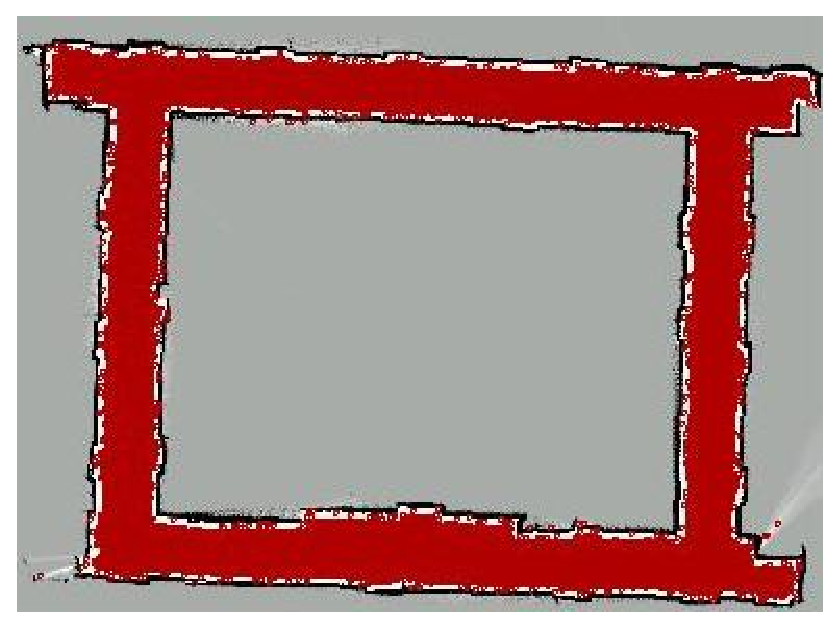
\epsfig{height=4cm,file=drivers/amcl-phe200-0010.eps} &
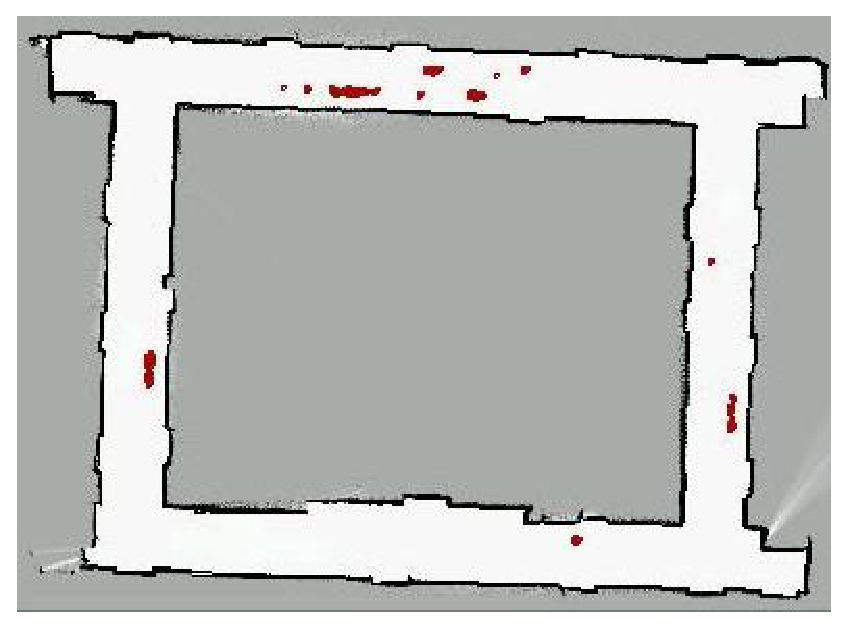
\epsfig{height=4cm,file=drivers/amcl-phe200-0400.eps} \\
$t = 10$~sec, $\approx 100,000$ particles & $t = 10$~sec, $\approx 1,000$ particles \\
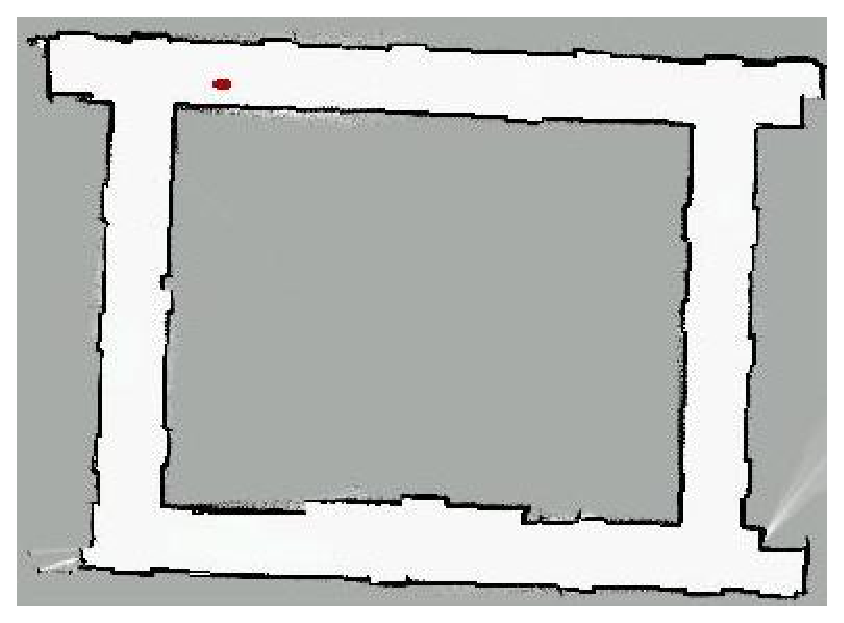
\epsfig{height=4cm,file=drivers/amcl-phe200-0800.eps} &
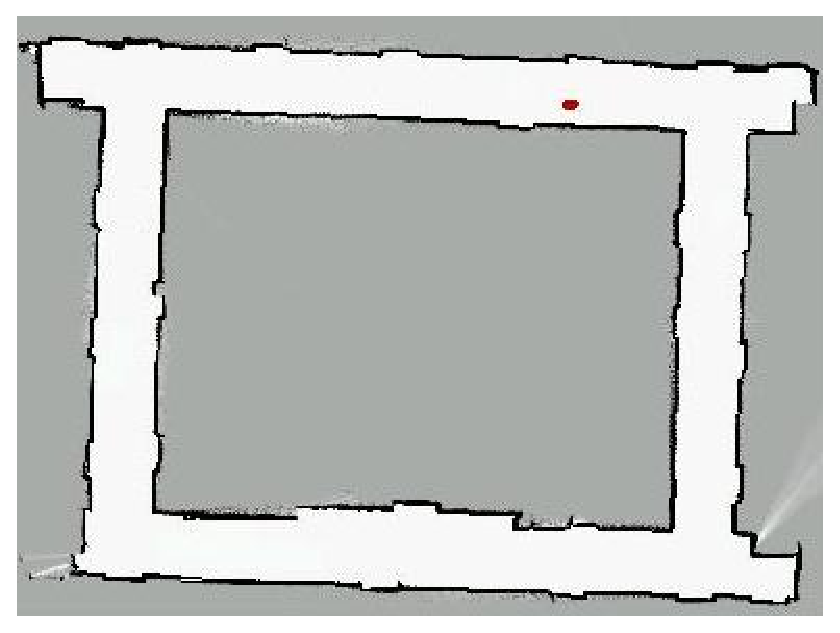
\epsfig{height=4cm,file=drivers/amcl-phe200-1200.eps} \\
$t = 80$~sec, $\approx 100$ particles & $t = 120$~sec, $\approx 100$ particles
\end{tabular}
\caption{Snap-shots showing the {\tt amcl} driver in action;
convergence in this case is relatively slow.}
\label{fig.amcl.example}
\end{center}
\end{figure*}


\subsection*{Caveats} 

At the time of writing, this driver is still evolving.  The sensor
models, in particular, are currently over-simplified and
under-parameterized (there are lots of magic numbers lurking about the
place).  Consequently, while this driver is known to work for certain
hardware configurations (think Pioneer2DX with a SICKLMS200 laser
range-finder), other configurations may require some refinement of the
sensor models.


\subsection*{Interfaces}

\noindent Supported interfaces:
\begin{itemize}
\item {\tt localize}
\end{itemize}

\noindent Required devices:
\begin{itemize}
\item {\tt position}
\item Any combination of: {\tt sonar}, {\tt laser} and {\tt wifi}.
\end{itemize}

\noindent Supported configuration requests:
\begin{itemize}
\item None.
\end{itemize}


\subsection*{Configuration file options}

\begin{center}
{\small \begin{tabularx}{\columnwidth}{|l|l|c|X|}
\hline
Name & Type & Default & Meaning\\
\hline

{\tt position\_index} & integer & 0 & Index of the position device to
use (this will usually be an odometric device of some sort). \\

{\tt sonar\_index} & integer & -1 & Index of the sonar ranging device
to use; set this to -1 if you dont wish to use sonar. \\

{\tt laser\_index} & integer & -1 & Index of the laser ranging device
to use; set this to -1 if you dont wish to use laser. \\

{\tt wifi\_index} & integer & -1 & Index of the WiFi signal-strength device
to use; set this to -1 if you dont wish to use WiFi signal-strength. \\

% Map options
{\tt map\_file} & filename & NULL & Name of the file containing the
occupancy map; see notes below for more on the map format. \\

{\tt map\_scale} & length & 0.05 & Scale of the map (meters/pixel). \\

{\tt map\_negate} & integer & 0 & Invert the states in the map
(occupied becomes empty and empty becomes occupied); see notes below. \\

% Odometic model
{\tt robot\_radius} & length & 0.20 & Effective radius of the robot
(meters); this value will be used to eliminate hypotheses that imply
that the robot is co-located with an obstacle. \\

% Sonar model

% Laser model
{\tt laser\_max\_samples} & integer & 5 & The maximum number of laser
range readings to use when updating the filter. \\

% WiFi model
{\tt wifi\_beacon\_N} & tuple & none & A tuple \verb+ [ "hostname"
"mapfilename" ]+ describing the $N^{\mathrm{th}}$ WiFi beacon.
{\tt hostname} specifies the name or IP address of the beacon; {\tt
mapfilename} points to the WiFi signal strength map for this
beacon. \\

% Particle filter
{\tt pf\_min\_samples} & integer & 100 & Lower bound on the number of
samples to maintain in the particle filter. \\

{\tt pf\_max\_samples} & integer & 10000 & Upper bound on the number of
samples to maintain in the particle filter. \\

{\tt pf\_err} & float & 0.01 & Control parameter for the particle set
size.  See notes below. \\

{\tt pf\_z} & float & 3 & Control parameter for the particle set
size.  See notes below. \\

% Initial conditions
{\tt init\_pose} & vector & [0 0 0] & Initial pose estimate (mean
value) for the robot (meters, meters, degrees). \\

{\tt init\_pose\_var} & vector & $[10^3 10^3 10^2]$ & Uncertainty in the
initial pose estimate (meters, meters, degrees). \\

% Debugging
{\tt enable\_gui} & integer & 0 & Set this to 1 to enable the built-in
driver GUI (useful for debugging).  Player must also be build with
{\tt configure --enable-rtkgui} for this option to have any effect. \\

\hline
\end{tabularx}}
\end{center}

\subsection*{Notes}

\begin{itemize}

\item {\bf Maps} 

The odometric, sonar and laser sensor models make use of a common
occupancy grid map.  This map is a regular grid in which cells are in
one of three states: occupied, empty or unknown (although the behavior
for unknown cells is currently undefined).  Maps are stored as
(uncompressed) images in PGM or PNM/grayscale format: black pixels are
treated as occupied cells, white pixels are treated as empty cells,
and the remaining colors are treated as unknown.  The interpretation
of these colors may be reversed (white is occupied, black is unknown)
by setting the {\tt map\_negate} flag in the configuration file.  This
flag is particularly handy if you wish to use the same image file as
both a map and a Stage bitmap.

TODO: WiFi maps

\item {\bf Coordinate System}

The origin of the global coordinate system corresponds to the center
of occupancy grid map.  Standard coordinate orientation is used; i.e.,
positive $x$ is towards the right of the map, positive $y$ towards the
top of the map.

\item {\bf Number of particles} 

The number of particles in the filter can be controlled using the
configuration file parameters {\tt pf\_err} and {\tt pf\_z}.
Specifically, {\tt pf\_err} is the maximum allowed error between the
true distribution and the estimated distribution, while {\tt pf\_z} is
the upper standard normal quantile for $(1 - p)$, where $p$ is the
probability that the error on the estimated distribution will be less
than {\tt pf\_err}.  If you dont know what that means, dont worry, I'm
not exactly sure either.  See \cite{fox01a} for a more meaningful
explanation.

\item {\bf Speed}

Many factors affect the speed at which the {\tt amcl} driver
runs, but the following tips might be helpful:
  \begin{itemize} 
  \item Reducing the number of laser range readings being used ({\tt
  laser\_max\_samples} in the configuration file) will significantly
  increase driver speed, but may also lead to slower convergence
  and/or less accurate localization.
  \item Increasing the allowed error {\tt pf\_err} and reducing the
  quantile {\tt pf\_z} will lead to smaller particle sets and will
  hence increase driver speed.  This may also lead, however, to
  over-convergence.
  \end{itemize}
As a benchmark, this driver has been successfully deployed on a
Pioneer2DX equipped with a SICK LMS200 and a 266MHz Mobile Pentium
with 32Mb of RAM.

\item {\bf Memory}

The two key factors affecting memory usage are:
  \begin{itemize}
  \item The size and resolution of the map.
  \item The maximum number of particles.
  \end{itemize}
As currently configured, the {\tt amcl} driver will typically use 10
to 20Mb of memory.  On embedded systems, where memory is at a premium,
users may have to decrease the map resolution or the maximum number of
particles to achieve acceptable preformance.


\end{itemize}




\subsection*{Example: Using the {\tt amcl} driver with a Pioneer robot}

The following configuration file illustrates the use of the {\tt
amcl} driver on a Pioneer robot equipped with a SICK LMS200
scanning laser range finder:
  \begin{small}
  \begin{verbatim}
  position:0 
  (
     driver "p2os_position" 
     port "/dev/ttyS1"
  )
  
  laser:0 
  (
    driver "sicklms200" 
    port "/dev/ttyS2"
  )

  localize:0 
  (
    driver "amcl"
    position_index 0
    laser_index 0
    map_file "mymap.pgm"
    map_scale 0.05
  )
  \end{verbatim}
  \end{small}
Naturally, the {\tt port}, {\tt map\_file} and {\tt map\_scale} values
should be changed to match your particular configuration.


\subsection*{Example: Using the {\tt amcl} driver with Stage}

The {\tt amcl} driver is not supported natively in Stage.
Users must therefore employ a second Player server configured to use
the {\tt passthrough} driver (see Section
\ref{sect:passthrough_driver}).  The basic procedure is as follows.
%
\begin{itemize}
\item Start Stage with a world file something like this:
  \begin{small}
  \begin{verbatim}
  ...
  position (port 6665 laser ())
  ...
  \end{verbatim}
  \end{small}
Stage will create one robot (position device) with a laser, and create
a Player server on port 6665.
\item Start another Player server using the command
  \begin{verbatim}
  player -p 7000 amcl.cfg
  \end{verbatim}
where the configuration file {\tt amcl.cfg} looks like this:
  \begin{small}
  \begin{verbatim}
  position:0 
  (
    driver "passthrough" 
    port 6665 index 0
  )

  laser:0 
  (
    driver "passthrough" 
    port 6665 
    index 0
  ) 

  localize:0 
  (
    driver "amcl" 
    position_index 0 
    laser_index 0 
    map_file "cave.pnm"
    map_scale 0.03
    map_negate 1
  )
  \end{verbatim}
  \end{small}
The second Player server will listen on port 7000; clients connecting
to this server will see a robot with {\tt position}, {\tt laser} and
{\tt localize} devices.  The map file {\tt cave.pnm} can be the same
file used by Stage to create the world bitmap.
\end{itemize}



\subsection*{Example: Using WiFi signal strength}

TODO


